% Options for packages loaded elsewhere
\PassOptionsToPackage{unicode}{hyperref}
\PassOptionsToPackage{hyphens}{url}
%
\documentclass[
  ignorenonframetext,
]{beamer}
\usepackage{pgfpages}
\setbeamertemplate{caption}[numbered]
\setbeamertemplate{caption label separator}{: }
\setbeamercolor{caption name}{fg=normal text.fg}
\beamertemplatenavigationsymbolsempty
% Prevent slide breaks in the middle of a paragraph
\widowpenalties 1 10000
\raggedbottom
\setbeamertemplate{part page}{
  \centering
  \begin{beamercolorbox}[sep=16pt,center]{part title}
    \usebeamerfont{part title}\insertpart\par
  \end{beamercolorbox}
}
\setbeamertemplate{section page}{
  \centering
  \begin{beamercolorbox}[sep=12pt,center]{part title}
    \usebeamerfont{section title}\insertsection\par
  \end{beamercolorbox}
}
\setbeamertemplate{subsection page}{
  \centering
  \begin{beamercolorbox}[sep=8pt,center]{part title}
    \usebeamerfont{subsection title}\insertsubsection\par
  \end{beamercolorbox}
}
\AtBeginPart{
  \frame{\partpage}
}
\AtBeginSection{
  \ifbibliography
  \else
    \frame{\sectionpage}
  \fi
}
\AtBeginSubsection{
  \frame{\subsectionpage}
}
\usepackage{amsmath,amssymb}
\usepackage{iftex}
\ifPDFTeX
  \usepackage[T1]{fontenc}
  \usepackage[utf8]{inputenc}
  \usepackage{textcomp} % provide euro and other symbols
\else % if luatex or xetex
  \usepackage{unicode-math} % this also loads fontspec
  \defaultfontfeatures{Scale=MatchLowercase}
  \defaultfontfeatures[\rmfamily]{Ligatures=TeX,Scale=1}
\fi
\usepackage{lmodern}
\usetheme[]{Madrid}
\ifPDFTeX\else
  % xetex/luatex font selection
\fi
% Use upquote if available, for straight quotes in verbatim environments
\IfFileExists{upquote.sty}{\usepackage{upquote}}{}
\IfFileExists{microtype.sty}{% use microtype if available
  \usepackage[]{microtype}
  \UseMicrotypeSet[protrusion]{basicmath} % disable protrusion for tt fonts
}{}
\makeatletter
\@ifundefined{KOMAClassName}{% if non-KOMA class
  \IfFileExists{parskip.sty}{%
    \usepackage{parskip}
  }{% else
    \setlength{\parindent}{0pt}
    \setlength{\parskip}{6pt plus 2pt minus 1pt}}
}{% if KOMA class
  \KOMAoptions{parskip=half}}
\makeatother
\usepackage{xcolor}
\newif\ifbibliography
\usepackage{color}
\usepackage{fancyvrb}
\newcommand{\VerbBar}{|}
\newcommand{\VERB}{\Verb[commandchars=\\\{\}]}
\DefineVerbatimEnvironment{Highlighting}{Verbatim}{commandchars=\\\{\}}
% Add ',fontsize=\small' for more characters per line
\usepackage{framed}
\definecolor{shadecolor}{RGB}{248,248,248}
\newenvironment{Shaded}{\begin{snugshade}}{\end{snugshade}}
\newcommand{\AlertTok}[1]{\textcolor[rgb]{0.94,0.16,0.16}{#1}}
\newcommand{\AnnotationTok}[1]{\textcolor[rgb]{0.56,0.35,0.01}{\textbf{\textit{#1}}}}
\newcommand{\AttributeTok}[1]{\textcolor[rgb]{0.13,0.29,0.53}{#1}}
\newcommand{\BaseNTok}[1]{\textcolor[rgb]{0.00,0.00,0.81}{#1}}
\newcommand{\BuiltInTok}[1]{#1}
\newcommand{\CharTok}[1]{\textcolor[rgb]{0.31,0.60,0.02}{#1}}
\newcommand{\CommentTok}[1]{\textcolor[rgb]{0.56,0.35,0.01}{\textit{#1}}}
\newcommand{\CommentVarTok}[1]{\textcolor[rgb]{0.56,0.35,0.01}{\textbf{\textit{#1}}}}
\newcommand{\ConstantTok}[1]{\textcolor[rgb]{0.56,0.35,0.01}{#1}}
\newcommand{\ControlFlowTok}[1]{\textcolor[rgb]{0.13,0.29,0.53}{\textbf{#1}}}
\newcommand{\DataTypeTok}[1]{\textcolor[rgb]{0.13,0.29,0.53}{#1}}
\newcommand{\DecValTok}[1]{\textcolor[rgb]{0.00,0.00,0.81}{#1}}
\newcommand{\DocumentationTok}[1]{\textcolor[rgb]{0.56,0.35,0.01}{\textbf{\textit{#1}}}}
\newcommand{\ErrorTok}[1]{\textcolor[rgb]{0.64,0.00,0.00}{\textbf{#1}}}
\newcommand{\ExtensionTok}[1]{#1}
\newcommand{\FloatTok}[1]{\textcolor[rgb]{0.00,0.00,0.81}{#1}}
\newcommand{\FunctionTok}[1]{\textcolor[rgb]{0.13,0.29,0.53}{\textbf{#1}}}
\newcommand{\ImportTok}[1]{#1}
\newcommand{\InformationTok}[1]{\textcolor[rgb]{0.56,0.35,0.01}{\textbf{\textit{#1}}}}
\newcommand{\KeywordTok}[1]{\textcolor[rgb]{0.13,0.29,0.53}{\textbf{#1}}}
\newcommand{\NormalTok}[1]{#1}
\newcommand{\OperatorTok}[1]{\textcolor[rgb]{0.81,0.36,0.00}{\textbf{#1}}}
\newcommand{\OtherTok}[1]{\textcolor[rgb]{0.56,0.35,0.01}{#1}}
\newcommand{\PreprocessorTok}[1]{\textcolor[rgb]{0.56,0.35,0.01}{\textit{#1}}}
\newcommand{\RegionMarkerTok}[1]{#1}
\newcommand{\SpecialCharTok}[1]{\textcolor[rgb]{0.81,0.36,0.00}{\textbf{#1}}}
\newcommand{\SpecialStringTok}[1]{\textcolor[rgb]{0.31,0.60,0.02}{#1}}
\newcommand{\StringTok}[1]{\textcolor[rgb]{0.31,0.60,0.02}{#1}}
\newcommand{\VariableTok}[1]{\textcolor[rgb]{0.00,0.00,0.00}{#1}}
\newcommand{\VerbatimStringTok}[1]{\textcolor[rgb]{0.31,0.60,0.02}{#1}}
\newcommand{\WarningTok}[1]{\textcolor[rgb]{0.56,0.35,0.01}{\textbf{\textit{#1}}}}
\usepackage{graphicx}
\makeatletter
\def\maxwidth{\ifdim\Gin@nat@width>\linewidth\linewidth\else\Gin@nat@width\fi}
\def\maxheight{\ifdim\Gin@nat@height>\textheight\textheight\else\Gin@nat@height\fi}
\makeatother
% Scale images if necessary, so that they will not overflow the page
% margins by default, and it is still possible to overwrite the defaults
% using explicit options in \includegraphics[width, height, ...]{}
\setkeys{Gin}{width=\maxwidth,height=\maxheight,keepaspectratio}
% Set default figure placement to htbp
\makeatletter
\def\fps@figure{htbp}
\makeatother
\setlength{\emergencystretch}{3em} % prevent overfull lines
\providecommand{\tightlist}{%
  \setlength{\itemsep}{0pt}\setlength{\parskip}{0pt}}
\setcounter{secnumdepth}{-\maxdimen} % remove section numbering
\logo{
\includegraphics[height=1cm,width=3cm]{logo.png}}
\usetheme{Madrid}
\usefonttheme{serif}
\setbeamertemplate{navigation symbols}{}
\usepackage{lmodern}  % for bold teletype font
\usepackage{amsmath}  % for \hookrightarrow
\usepackage{xcolor}   % for \textcolor


\ifLuaTeX
  \usepackage{selnolig}  % disable illegal ligatures
\fi
\usepackage{bookmark}
\IfFileExists{xurl.sty}{\usepackage{xurl}}{} % add URL line breaks if available
\urlstyle{same}
\hypersetup{
  pdftitle={Leksioni 11},
  pdfauthor={Endri Raco},
  hidelinks,
  pdfcreator={LaTeX via pandoc}}

\title{Leksioni 11}
\author{Endri Raco}
\date{24 May, 2024}

\begin{document}
\frame{\titlepage}

\begin{frame}[allowframebreaks]
  \tableofcontents[hideallsubsections]
\end{frame}
\section{Hyrje në SQL}\label{hyrje-nuxeb-sql}

\begin{frame}{Si të Shkarkoni dhe Instaloni Mjetet e SQLite}
\phantomsection\label{si-tuxeb-shkarkoni-dhe-instaloni-mjetet-e-sqlite}
\begin{itemize}
\item
  Shko në faqen zyrtare: \url{https://www.sqlite.org}
\item
  Hap faqen e shkarkimit: \url{https://www.sqlite.org/download.html}
\end{itemize}
\end{frame}

\begin{frame}{Si të Shkarkoni dhe Instaloni Mjetet e SQLite}
\phantomsection\label{si-tuxeb-shkarkoni-dhe-instaloni-mjetet-e-sqlite-1}
Zgjidh dhe shkarko versionin përkatës për sistemin tënd operativ (p.sh.,
Windows, x64 ose x86)

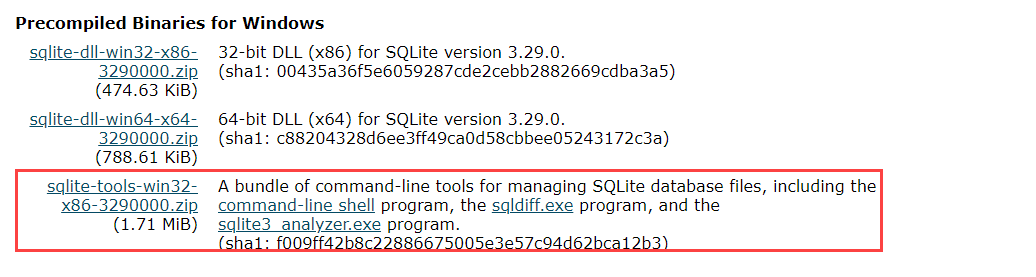
\includegraphics{./Figs/sql.png}
\end{frame}

\begin{frame}{Instalimi i Mjeteve SQLite}
\phantomsection\label{instalimi-i-mjeteve-sqlite}
\begin{itemize}
\item
  Krijo një dosje të re, p.sh \textbf{sqlite}
\item
  Ekstrakto përmbajtjen e skedarit të shkarkuar në këtë dosje
\end{itemize}

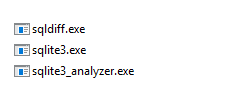
\includegraphics{./Figs/sql2.png}
\end{frame}

\begin{frame}{Ekzekutimi i SQLite nga Command Line}
\phantomsection\label{ekzekutimi-i-sqlite-nga-command-line}
\begin{itemize}
\tightlist
\item
  Hap dritaren e Command Line
\end{itemize}

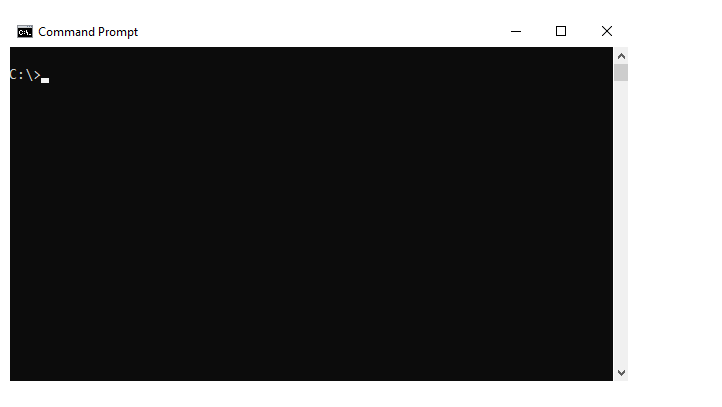
\includegraphics{./Figs/sql3.png}
\end{frame}

\begin{frame}{Ekzekutimi i SQLite nga Command Line}
\phantomsection\label{ekzekutimi-i-sqlite-nga-command-line-1}
\begin{itemize}
\tightlist
\item
  Navigo në dosjen \textbf{sqlite}
\end{itemize}

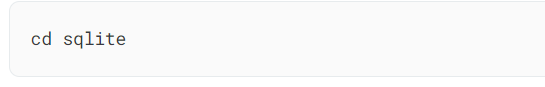
\includegraphics{./Figs/sql4.png}
\end{frame}

\begin{frame}{Ekzekutimi i SQLite nga Command Line}
\phantomsection\label{ekzekutimi-i-sqlite-nga-command-line-2}
\begin{itemize}
\tightlist
\item
  Ekzekuto SQLite duke shkruar: sqlite3
\end{itemize}
\end{frame}

\begin{frame}{Instalimi dhe Përdorimi i SQLiteStudio}
\phantomsection\label{instalimi-dhe-puxebrdorimi-i-sqlitestudio}
\begin{itemize}
\tightlist
\item
  Tani shohim hap pas hapi se si të instaloni dhe përdorni SQLiteStudio,
  një mjet falas dhe intuitiv GUI për menaxhimin e bazave të të dhënave
  SQLite.
\end{itemize}
\end{frame}

\begin{frame}[fragile]{Shkarkimi i SQLiteStudio}
\phantomsection\label{shkarkimi-i-sqlitestudio}
SQLiteStudio është një mjet GUI falas dhe i lehtë për t'u përdorur që
mund të shkarkohet nga faqja zyrtare.

\begin{enumerate}
\item
  Hapni faqen e internetit
  \url{https://github.com/pawelsalawa/sqlitestudio/releases}.
\item
  Zgjidhni versionin që dëshironi të shkarkoni, siç është versioni i
  instaluesit ose versioni portativ.
\item
  Ruajeni skedarin e shkarkuar në një dosje në kompjuterin tuaj, për
  shembull
  \texttt{C:\textbackslash{}\textbackslash{}sqlite\textbackslash{}\textbackslash{}gui}.
\end{enumerate}
\end{frame}

\begin{frame}{Instalimi i SQLiteStudio}
\phantomsection\label{instalimi-i-sqlitestudio}
Pas shkarkimit, ndiqni këto hapa për të instaluar SQLiteStudio:

\begin{enumerate}
\item
  Navigoni tek dosja ku keni ruajtur skedarin e shkarkuar.
\item
  Ekstraktoni përmbajtjen e skedarit ZIP nëse keni shkarkuar versionin
  portativ.
\item
  Nëse keni shkarkuar instaluesin, klikoni dyfish mbi të për të filluar
  procesin e instalimit dhe ndiqni udhëzimet në ekran.
\end{enumerate}
\end{frame}

\begin{frame}[fragile]{Nisja e SQLiteStudio}
\phantomsection\label{nisja-e-sqlitestudio}
Për të hapur SQLiteStudio pas instalimit:

\begin{enumerate}
\item
  Shkoni tek dosja ku e keni instaluar programin, për shembull
  \texttt{C:\textbackslash{}\textbackslash{}sqlite\textbackslash{}\textbackslash{}gui\textbackslash{}\textbackslash{}SQLiteStudio}.
\item
  Klikoni dy herë mbi ikonën e SQLiteStudio për ta hapur programin.
\end{enumerate}
\end{frame}

\begin{frame}{Hyrje në SQL Server}
\phantomsection\label{hyrje-nuxeb-sql-server}
\begin{itemize}
\tightlist
\item
  SQL Server është një sistem databaze relacionale të zhvilluar nga
  Microsoft.
\end{itemize}
\end{frame}

\begin{frame}{Hyrje në SQL Server}
\phantomsection\label{hyrje-nuxeb-sql-server-1}
Do mësojmë:

\begin{itemize}
\item
  Si të shkruani pyetje (queries)
\item
  Konceptet bazë të SQL Server
\end{itemize}
\end{frame}

\begin{frame}{Hyrje në SQL Server}
\phantomsection\label{hyrje-nuxeb-sql-server-2}
\begin{itemize}
\item
  SQL Server është \textbf{dyqani} që përmban bazat e të dhënave dhe
  tabelat
\item
  \textbf{Queries} janë mënyra si i marrim \textbf{produktet} nga
  \textbf{raftet} dhe ngarkojmë \textbf{koshin}
\item
  \textbf{SELECT} është termi kyç për të marrë të dhëna
\end{itemize}
\end{frame}

\section{Si të Importoni një Skedar CSV në
SQLiteStudio}\label{si-tuxeb-importoni-njuxeb-skedar-csv-nuxeb-sqlitestudio}

\begin{frame}{Hapi 1: Hapni SQLiteStudio}
\phantomsection\label{hapi-1-hapni-sqlitestudio}
\begin{itemize}
\tightlist
\item
  Hapni SQLiteStudio në kompjuterin tuaj.
\end{itemize}
\end{frame}

\begin{frame}[fragile]{Hapi 2: Krijoni ose Hapni një Bazë të Të Dhënave}
\phantomsection\label{hapi-2-krijoni-ose-hapni-njuxeb-bazuxeb-tuxeb-tuxeb-dhuxebnave}
Nëse nuk keni një bazë të të dhënave ku do të importoni CSV-në, krijoni
një të re:

\begin{itemize}
\item
  Shkoni te menuja \textbf{Database} dhe zgjidhni \textbf{Add a
  database}.
\item
  Zgjidhni një emër për bazën e të dhënave (p.sh.,
  \texttt{MyDatabase.db}) dhe vendndodhjen, më pas klikoni \textbf{OK}.
\end{itemize}
\end{frame}

\begin{frame}{Hapi 2: Krijoni ose Hapni një Bazë të Të Dhënave}
\phantomsection\label{hapi-2-krijoni-ose-hapni-njuxeb-bazuxeb-tuxeb-tuxeb-dhuxebnave-1}
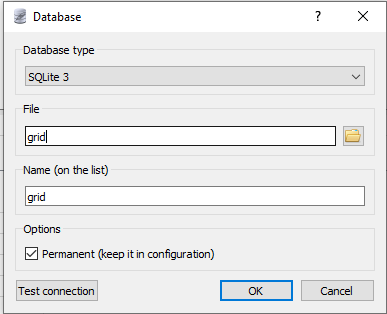
\includegraphics{./Figs/sql7.png}
\end{frame}

\begin{frame}{Hapi 2: Krijoni ose Hapni një Bazë të Të Dhënave}
\phantomsection\label{hapi-2-krijoni-ose-hapni-njuxeb-bazuxeb-tuxeb-tuxeb-dhuxebnave-2}
\begin{itemize}
\item
  Nëse tashmë keni një bazë të të dhënave, sigurohuni që ajo është e
  hapur në SQLiteStudio.
\item
  Krijoni lidhjen me databazën.
\end{itemize}

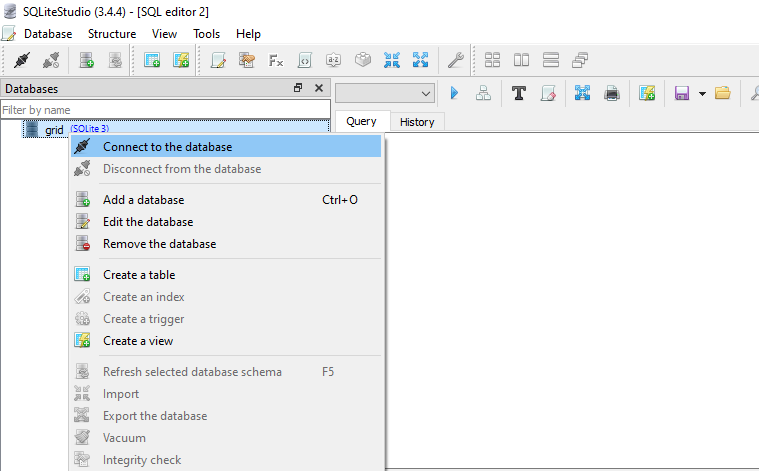
\includegraphics{./Figs/sql8.png}
\end{frame}

\begin{frame}{Hapi 3: Importoni Skedarin CSV}
\phantomsection\label{hapi-3-importoni-skedarin-csv}
\begin{itemize}
\tightlist
\item
  Me bazën e të dhënave të hapur, shkoni te menuja \textbf{Tools} dhe
  zgjidhni \textbf{Import}.
\end{itemize}

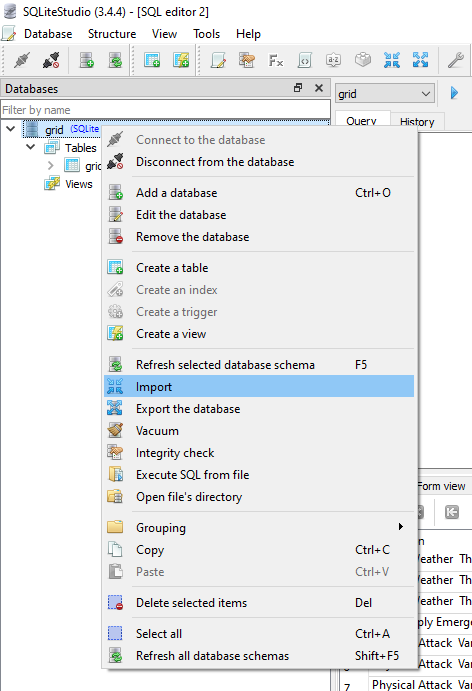
\includegraphics{./Figs/sql10.png}
\end{frame}

\begin{frame}{Hapi 3: Importoni Skedarin CSV}
\phantomsection\label{hapi-3-importoni-skedarin-csv-1}
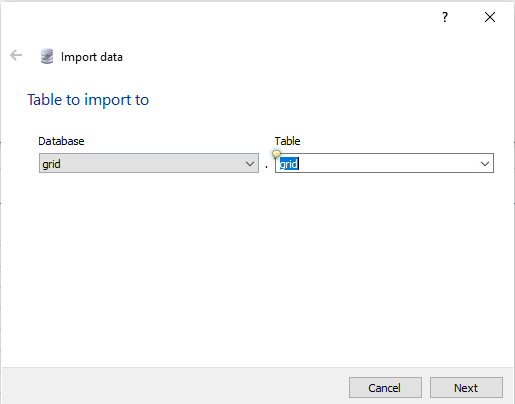
\includegraphics{./Figs/sql11.png}
\end{frame}

\begin{frame}{Hapi 3: Importoni Skedarin CSV}
\phantomsection\label{hapi-3-importoni-skedarin-csv-2}
\begin{itemize}
\tightlist
\item
  Në dritaren e importit, zgjidhni \textbf{CSV} si formatin dhe klikoni
  \textbf{Next}.
\end{itemize}

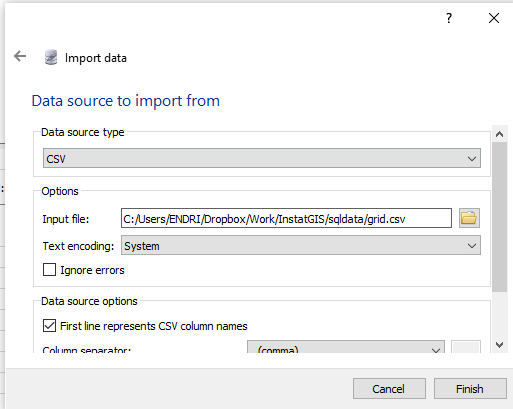
\includegraphics{./Figs/sql12.png}
\end{frame}

\begin{frame}{Hapi 4: Konfiguroni Importimin e CSV-së}
\phantomsection\label{hapi-4-konfiguroni-importimin-e-csv-suxeb}
\begin{itemize}
\item
  Shfletoni për të gjetur skedarin CSV që dëshironi të importoni.
\item
  Pasi ta zgjidhni skedarin tuaj CSV, do të kërkoheni të konfiguroni
  cilësimet e importit:

  \begin{itemize}
  \item
    \textbf{Emri i tabelës}: Është zakonisht e zakonshme të emëroni
    tabelën pas skedarit CSV, pa prapashtesën e skedarit.
  \item
    \textbf{Emrat dhe llojet e kolonave}: SQLiteStudio do t'ju ofrojë
    mundësinë të konfiguroni kolonat duke përcaktuar emrat dhe llojet e
    të dhënave për secilën kolonë.
  \end{itemize}
\end{itemize}
\end{frame}

\begin{frame}{Hapi 5: Përfundo Importimin}
\phantomsection\label{hapi-5-puxebrfundo-importimin}
\begin{itemize}
\item
  Pas konfigurimit të cilësimeve, vazhdoni me importimin duke ndjekur
  udhëzimet në SQLiteStudio.
\item
  Kontrolloni të dhënat e importuara për të siguruar se janë saktë dhe
  siç pritej.
\end{itemize}
\end{frame}

\begin{frame}[fragile]{Fillojmë}
\phantomsection\label{fillojmuxeb}
\begin{itemize}
\item
  \textbf{SELECT} është termi kyç për të marrë të dhëna
\item
  Shembull: \texttt{SELECT\ description\ FROM\ grid;}
\end{itemize}
\end{frame}

\begin{frame}{Anatomia e një pyetjeje të thjeshtë SELECT}
\phantomsection\label{anatomia-e-njuxeb-pyetjeje-tuxeb-thjeshtuxeb-select}
\begin{itemize}
\item
  Deklaratat \textbf{SELECT} specifikojnë atë që duam të marrim nga një
  tabelë.
\item
  Query më e thjeshtë zgjedh një kolonë, nga një tabelë.
\end{itemize}
\end{frame}

\begin{frame}{Anatomia e një pyetjeje të thjeshtë SELECT}
\phantomsection\label{anatomia-e-njuxeb-pyetjeje-tuxeb-thjeshtuxeb-select-1}
\begin{itemize}
\tightlist
\item
  Në këtë query, ne zgjedhim shtyllën \textbf{description}, nga tabela
  \textbf{grid}.
\end{itemize}
\end{frame}

\begin{frame}{Anatomia e një pyetjeje të thjeshtë SELECT}
\phantomsection\label{anatomia-e-njuxeb-pyetjeje-tuxeb-thjeshtuxeb-select-2}
\begin{itemize}
\item
  Vini re pikëpresjen që tregon fundin e qyery-t.
\item
  Fjala tjetër kyçe që do t'ju duhet gjithmonë është \textbf{FROM} - për
  të specifikuar vendndodhjen e tabelës burimore.
\end{itemize}
\end{frame}

\begin{frame}[fragile]{Fillojmë}
\phantomsection\label{fillojmuxeb-1}
\AddToHookNext{env/Highlighting/begin}{\tiny}

\begin{Shaded}
\begin{Highlighting}[]
\KeywordTok{SELECT}\NormalTok{ description}
\KeywordTok{FROM}\NormalTok{ grid;}
\end{Highlighting}
\end{Shaded}
\end{frame}

\begin{frame}{Fillojmë}
\phantomsection\label{fillojmuxeb-2}
Këtu janë rezultatet. Query kthen çdo rresht në kolonën e zgjedhur.

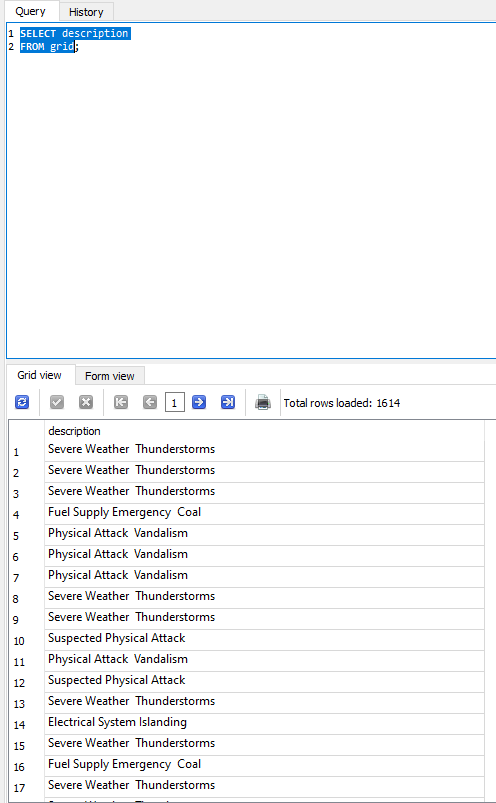
\includegraphics{./Figs/sql13.png}
\end{frame}

\begin{frame}{Praktikë}
\phantomsection\label{praktikuxeb}
\begin{itemize}
\item
  Përsëritni hapat e mësipërm për të lidhur një databazë \textbf{artist}
\item
  Do përdorim skedarin csv \textbf{artist} nga folder \textbf{db}
\end{itemize}
\end{frame}

\begin{frame}{Query me më shumë se një kolonë}
\phantomsection\label{query-me-muxeb-shumuxeb-se-njuxeb-kolonuxeb}
\begin{itemize}
\item
  Ju mund të zgjidhni kolona të shumta, duke e ndarë çdo emër kolone me
  një presje.
\item
  Nuk keni nevojë për presje për kolonën e fundit të zgjedhur përpara
  `FROM'.
\end{itemize}
\end{frame}

\begin{frame}{Query me më shumë se një kolonë}
\phantomsection\label{query-me-muxeb-shumuxeb-se-njuxeb-kolonuxeb-1}
\begin{itemize}
\tightlist
\item
  Sigurohemi që kemi bërë \textbf{disconnect} nga databaza
  \textbf{artist}
\end{itemize}
\end{frame}

\begin{frame}[fragile]{Zgjedhja e më shumë se një kolone}
\phantomsection\label{zgjedhja-e-muxeb-shumuxeb-se-njuxeb-kolone}
\AddToHookNext{env/Highlighting/begin}{\tiny}

\begin{Shaded}
\begin{Highlighting}[]
\KeywordTok{SELECT}\NormalTok{ artistId, Name}
\KeywordTok{FROM}\NormalTok{ artist;}
\end{Highlighting}
\end{Shaded}
\end{frame}

\begin{frame}{Formatimi i Query}
\phantomsection\label{formatimi-i-query}
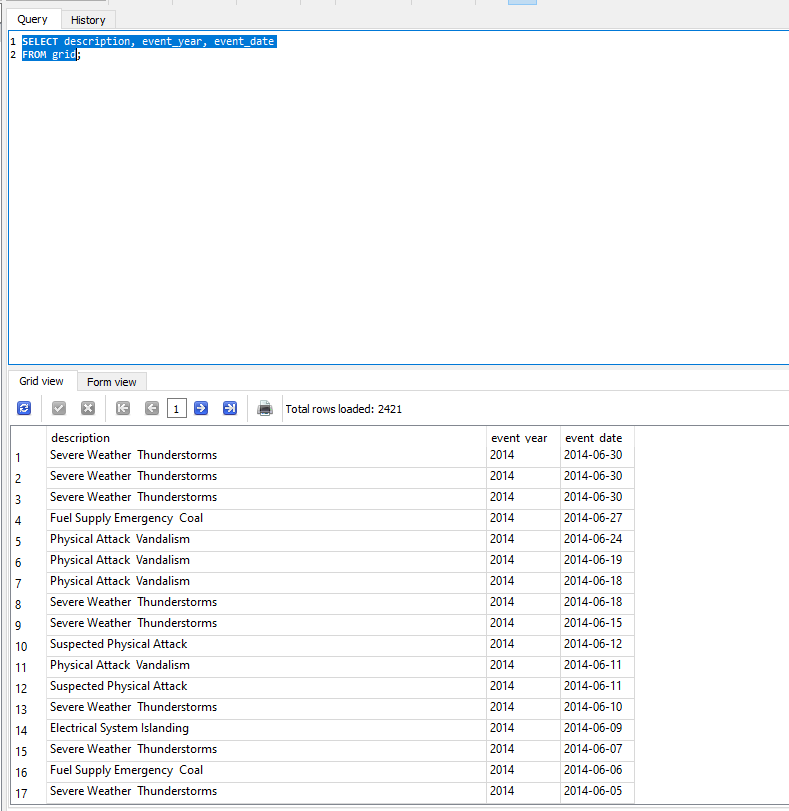
\includegraphics{./Figs/sql14.png}
\end{frame}

\begin{frame}{Formatimi i Query}
\phantomsection\label{formatimi-i-query-1}
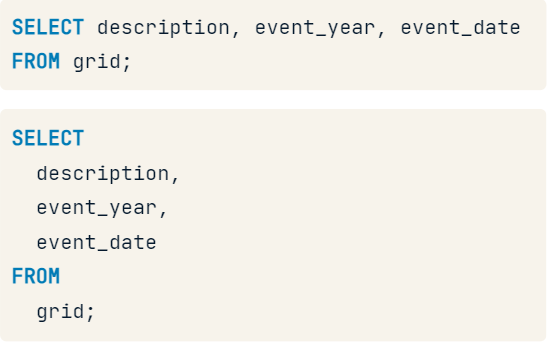
\includegraphics{./Figs/sql15.png}
\end{frame}

\begin{frame}{Formatimi i Query}
\phantomsection\label{formatimi-i-query-2}
\begin{itemize}
\item
  Këtu janë 2 query të ngjashme, me paraqitje të ndryshme.
\item
  Query e sipërme tregon të gjitha kolonat që do të zgjidhen në një
  rresht.
\item
  Query e poshtme tregon çdo kolonë të zgjedhur në një rresht të ri.
\end{itemize}
\end{frame}

\begin{frame}{Formatimi i Query}
\phantomsection\label{formatimi-i-query-3}
\begin{itemize}
\item
  Rezultatet e të dy query-ve do të jenë identike.
\item
  Ne do të përdorim kryesisht paraqitjen e poshtme gjatë gjithë
  leksioneve.
\end{itemize}
\end{frame}

\begin{frame}{Formatimi i Query}
\phantomsection\label{formatimi-i-query-4}
Mbajtja e fjalëve kyçe si SELECT dhe FROM me shkronja të mëdha, dhe
emrat e tabelave dhe kolonave me shkronja të vogla, i bën query më të
lehta për t'u lexuar.
\end{frame}

\begin{frame}[fragile]{Formatimi i Query}
\phantomsection\label{formatimi-i-query-5}
\AddToHookNext{env/Highlighting/begin}{\tiny}

\begin{Shaded}
\begin{Highlighting}[]
\KeywordTok{SELECT} 
\NormalTok{  description, }
\NormalTok{  event\_year, }
\NormalTok{  event\_date}
\KeywordTok{FROM} 
\NormalTok{  grid;}
\end{Highlighting}
\end{Shaded}
\end{frame}

\begin{frame}{Formatimi i Query}
\phantomsection\label{formatimi-i-query-6}
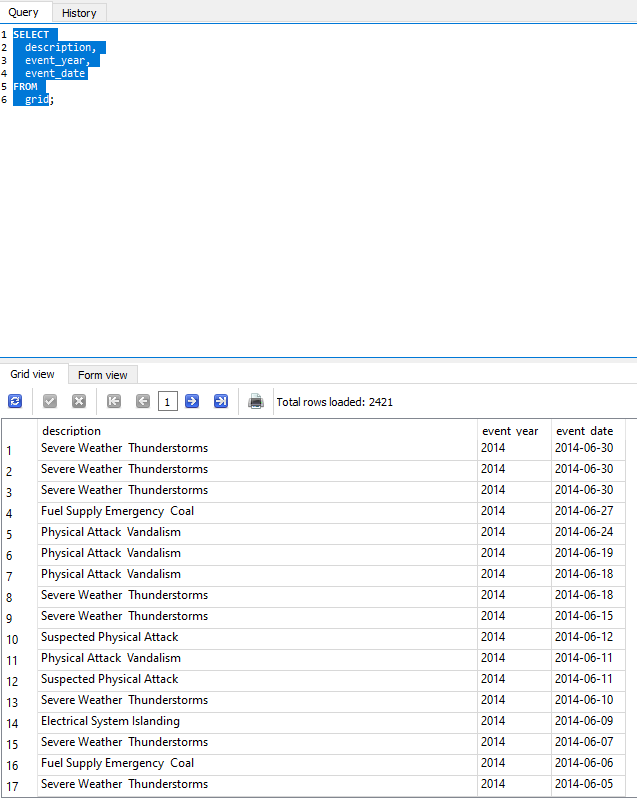
\includegraphics{./Figs/sql16.png}
\end{frame}

\end{document}
